% =========================================================================== %
% Yes. This is a document.

\documentclass[
	english,
	aspectratio=169,
	table
]{beamer}

% =========================================================================== %
% Theme
\usepackage{scrlfile}
	\ReplacePackage{beamerthemeSHUR}{./sty/beamerthemeSHUR}
	\ReplacePackage{beamerinnerthemefancy}{./sty/beamerinnerthemefancy}
	\ReplacePackage{beamerouterthemedecolines}{./sty/beamerouterthemedecolines}
	\ReplacePackage{beamercolorthemechameleon}{./sty/beamercolorthemechameleon}

\usetheme[
	pageofpages=von,
	bullet=circle,
	titleline=true,
	alternativetitlepage=true,
	watermark="",
	watermarkheight=0px,
	watermarkheightmult=0
	]
{SHUR}

% =========================================================================== %
% the usual stuff

\usepackage[utf8]{inputenc}
\usepackage[T1]{fontenc}
\usepackage{babel}
\usepackage{lmodern}
\usepackage{microtype}
\usepackage{csquotes}

\usepackage{tabularx}
\usepackage{booktabs}
\usepackage{multirow}

\usepackage{color, colortbl}
\usepackage{xcolor}
	\definecolor{tabhighlight}{RGB}{230,240,255}

\usepackage{tabto}

% math
\usepackage{amsmath}
\usepackage{amssymb}
\usepackage{dsfont}
\usepackage[arrowdel]{physics}
\usepackage{mathtools}

\usepackage{minted}
	\usemintedstyle{friendly}

\usepackage{tikz}
	\usetikzlibrary{positioning}
	\usetikzlibrary{matrix}
	\usetikzlibrary{shapes.geometric}
	\usetikzlibrary{backgrounds}
	\usetikzlibrary{calc}
	\usetikzlibrary{decorations.pathreplacing}
	\tikzstyle{every picture}+=[remember picture] 
\usepackage{adjustbox}

\usepackage[most]{tcolorbox}
	\tcbsetforeverylayer
		{colback=cyan!10!white,
		 colframe=cyan!75!black,
		 arc=0pt,
		 outer arc=0pt,
		 parbox=false
		}
	\newtcolorbox{codebox}[1][Code]
		{colback=black!5!white,
		 colframe=blue!40!black,
		 title=#1,
		 leftupper=6mm
		}
	\newtcolorbox{cmdbox}[1][Terminal]
		{colback=black,
		 coltext=white,
		 fontupper=\ttfamily ,
		 colframe=blue!40!black,
		 title=#1,
		 outer arc=0pt
		}
	\newtcolorbox{warnbox}[1][Attention]
		{colback=black!5!white,
		 colframe=red!40!black,
		 title=#1
		}
	\newtcolorbox{hintbox}[1][Hint]
		{colback=black!5!white,
		 colframe=green!40!black,
		 title=#1
		}
	\newenvironment{itembox}
		{\begin{tcolorbox}\begin{itemize}}%
		{\end{itemize}\end{tcolorbox}}
	\newtcolorbox{doublebox}[1][.3]
		{righthand width=#1\linewidth,
		 sidebyside,
		 sidebyside gap=6mm,
		 sidebyside align=center,
		 lower separated=false}
	
%==============================================================================%
% GLOBAL MACROS

\newcommand*{\eg}{e.\,g. }
\newcommand*{\ie}{i.\,e. }

\newcommand{\Thus}{\ensuremath{\Rightarrow}}
\newcommand{\thus}{\ensuremath{\rightarrow}}

\newcommand*{\tabcrlf}{\\ \midrule}			% actually still allows for optional argument

\newcommand*{\inPy}[1]{\mintinline{python}{#1}}

% =========================================================================== %

\author{Stefan Hartinger}
\title{Programming in Python}
\subtitle{Part 7: Advanced Techniques with Functions}
\institute{University Regensburg, Department of Theoretical Physics}
\date{Block Course, Summer Term 2021}

% =========================================================================== %

\begin{document}
% =========================================================================== %

\begin{frame}[t,plain]
\titlepage
\end{frame}

% =========================================================================== %

\begin{frame}{Recap}
%
\begin{columns}[T]
\column{.5\linewidth}
\begin{itemize}
\item \inPy{while}-loops
	\begin{itemize}
	\item Repeat code as long as (\emph{while}) a condition is satisfied
	\end{itemize}
\item \inPy{break} and \inPy{continue}
	\begin{itemize}
	\item Stop looping early (\inPy{break}) or skip part of the loop body (\inPy{continue})
	\end{itemize}
\item \inPy{else} with \inPy{for} and \inPy{while}
	\begin{itemize}
	\item execute code only when end of loop is reached
	\item skip over \inPy{else} clause with \inPy{break}
	\end{itemize}
\end{itemize}
%
\column{.5\linewidth}
\begin{itemize}
\item Functions
	\begin{itemize}
	\item Separate blocks of code
	\item New commands for doing larger blocks of work at once
	\item Variables local to the function\\
		(\thus scopes)
	\item Only \emph{mutable} variables can be changed by a function
	\item Memory model -- old references under new (local) names
	\end{itemize}
\end{itemize}

\end{columns}
%
\begin{center}
	\emph{Any Questions?}
\end{center}
%
\end{frame}

% =========================================================================== %

\begin{frame}[fragile]{Chapter 6}
%
\begin{itemize}
\item Optional Arguments
\item Variadic Functionens
\item Functions as return value
\item Lambdas
\item Recursion
\end{itemize}
%
\end{frame}

% =========================================================================== %

\begin{frame}[fragile]{Optional Arguments}
%
\begin{columns}[T]
\column{.45\linewidth}
\begin{itemize}
\item Recap: Functions allow doing recurrent tasks with a single call
\item Parametrised -- list of values used in execution of the task
\item Often: standard arguments, used almost every time
\item New syntax: render some arguments optional and define a default value
\item Lingu: \emph{positional} and \emph{optional} arguments
\end{itemize}
%
\column{.55\linewidth}
\begin{codebox}[Syntax: Optional Arguments]
\begin{minted}[fontsize=\scriptsize]{python}
def funcName (param, optParam = default) :
    ...
\end{minted}
\end{codebox}
%
\begin{codebox}[Syntax: Calling Functions with Optional Arguments]
\begin{minted}[fontsize=\scriptsize]{python}
funcName (param)
funcName (param, optParam)
\end{minted}
\end{codebox}
\end{columns}
%
\end{frame}

% =========================================================================== %

\begin{frame}[fragile]{Optional Arguments}
%
\begin{columns}[T]
\column{.5\linewidth}
\begin{itemize}
\item Arbitrary count of \emph{positional} (normal) arguments
\item Arbitrary count of optionals arguments
\item Optional arguments: always after positional arguments
\item In a call: can be only omitted \emph{from the end, backwards}
\end{itemize}
%
\column{.5\linewidth}
\begin{codebox}[Example: Call With opt. Arguments]
\begin{minted}[linenos, fontsize=\scriptsize]{python}
# def func (a, b = 2, c) :
#    ! last argument not optional!

def func (a, b = 2, c = 3) :
    print(a, b, c)
    
func(1)            # a= 1, b= 2, c= 3
func(-1, -2)       # a=-1, b=-2, c= 3
func(-1, -2, -3)   # a=-1, b=-2, c=-3
# func(-1, , -3)
#    ! cannot skip arguments!
\end{minted}
\end{codebox}
\end{columns}
%
\end{frame}

% =========================================================================== %

\begin{frame}[fragile]{Variadic Functions}
%
\begin{columns}[T]
\column{.5\linewidth}
\begin{itemize}
\item Some functions allow an arbitrary count of arguments in a call
\item Cf. \inPy{print}
\item New Syntax in function definition
	\begin{itemize}
	\item Asterisk (*) in front of \emph{one} argument
	\item By convention: \texttt{*args}
	\item Note: The asterisk is \emph{not} part of the variable name!
	\end{itemize}
\item Pass arguments as a \inPy{tuple}
\end{itemize}
%
\column{.5\linewidth}
\begin{codebox}[Syntax: Variadic Functions]
\begin{minted}[fontsize=\scriptsize]{python}
def funcName (params, *args) :
    ...
\end{minted}
\end{codebox}
%
\begin{codebox}[Syntax: Aufruf Variadische Fktn.]
\begin{minted}[fontsize=\scriptsize]{python}
funcName (param)
funcName (param, varArg1, varArg2, ...)
\end{minted}
\end{codebox}
\end{columns}
%
\end{frame}

% =========================================================================== %

\begin{frame}{Variadic Functions}
%
\begin{itemize}
\item Arbitrary count of positional arguments \emph{before} the variadic one
\item At most one variadic argument -- absorbs all variadic arguments
\item Arbitrary count of \emph{optional} arguments
	\begin{itemize}
	\item Both, before and after the variadic one
	\item Assignment via clause \inPy{optParam = Wert}
	\item Optional arguments \emph{cannot} be put in between variadic arguments
	\item See more to that in a minute
	\end{itemize}
\end{itemize}
%
\end{frame}

% =========================================================================== %

\begin{frame}[fragile]
%
\begin{tcbraster}[raster columns=2,
                  raster equal height,
                  nobeforeafter,
                  raster column skip=0.5cm]
\begin{codebox}[Example: Variadic Functions]
\begin{minted}[linenos, fontsize=\scriptsize]{python}
def func (
    posArg1, posArg2,
    *varArg,
    optArg = 0
) :
    print("pos. arguments:",
          posArg1, posArg2)
    print("var. argument :", varArg)
    print("opt. argument :", optArg)
    print()

func(1, 2)
func(1, 2, 3, 4, 5, 6, "seven")
func(1, 2, 3, optArg = 4)
func(1, 2, optArg = 3)
\end{minted}
\end{codebox}
%
\begin{cmdbox}[Output: Variadic Functions]
\begin{minted}[fontsize=\scriptsize]{text}
pos. arguments: 1 2
var. argument : ()
opt. argument : 0

pos. arguments: 1 2
var. argument : (3, 4, 5, 6, 'seven')
opt. argument : 0

pos. arguments: 1 2
var. argument : (3,)
opt. argument : 4

pos. arguments: 1 2
var. argument : ()
opt. argument : 3
\end{minted}
\end{cmdbox}
\end{tcbraster}
%
\end{frame}

% =========================================================================== %

\begin{frame}[fragile]{Keyword Arguments}
%
\begin{columns}[T]
\column{.5\linewidth}
\begin{itemize}
\item Similar to variadic arguments, but: pass pairs of key : value
\item New syntax in function definition: \texttt{**kwargs}
	\begin{itemize}
	\item By convention: \texttt{kwargs}
	\item Note that the asterisks are not part of the variable name
	\end{itemize}
\item New syntax in call: \inPy{funcName(..., key = value, ...)}
\item I.\,e. the same as just seen with \emph{optional keywords} after \emph{variadic keywords}
\item Passed on as \inPy{dict}
\end{itemize}
%
\column{.5\linewidth}
\begin{codebox}[Syntax: Variadische Funktionen]
\begin{minted}[fontsize=\scriptsize]{python}
def Funkname (params, **kwargs) :
    ...
\end{minted}
\end{codebox}
%
\begin{codebox}[Syntax: Aufruf Variadische Fktn.]
\begin{minted}[fontsize=\scriptsize]{python}
Funkname (par)
Funkname (par, kw1 = v1, kw2 = v2, ...)
\end{minted}
\end{codebox}
\end{columns}
%
\end{frame}

% =========================================================================== %

\begin{frame}[fragile]
%
\begin{tcbraster}[raster columns=2,
                  raster equal height,
                  nobeforeafter,
                  raster column skip=0.5cm]
\begin{codebox}[Example: Keyword Arguments]
\begin{minted}[linenos, fontsize=\scriptsize]{python}
def func (
    posArg1, posArg2,
    optArg = 0,
    *varArg, **kwArgs
) :
    print("pos. arguments:",
          posArg1, posArg2)
    print("var. argument   :", varArg)
    print("opt. argument   :", optArg)
    print("key. argument   :", kwArgs)
    print()

func(1, 2, 3)
func(1, 2, key="value")
func(1, 2, optArg="value")
# func(1, 2, 3, optArg="value")
#    ! multiple values for optArg!
func(1, 2, "value", 4, key="value")
\end{minted}
\end{codebox}
%
\begin{cmdbox}[Output: Keyword Arguments]
\begin{minted}[fontsize=\scriptsize]{text}
pos. arguments: 1 2
var. argument   : ()
opt. argument   : 3
key. argument   : {}

pos. arguments: 1 2
var. argument   : ()
opt. argument   : 0
key. argument   : {'key': 'value'}

pos. arguments: 1 2
var. argument   : ()
opt. argument   : value
key. argument   : {}

pos. arguments: 1 2
var. argument   : (4,)
opt. argument   : value
key. argument   : {'key': 'value'}
\end{minted}
\end{cmdbox}
\end{tcbraster}
%
\end{frame}

% =========================================================================== %

\begin{frame}{Keyword Arguments}
%
\begin{itemize}
\item Arbitrary many keyword-value pairs in calls
\item Only one keyword argument in the definition -- absorbs all keywords into a single \inPy{dict}
\end{itemize}
%
\begin{columns}[T]
\column{.4\linewidth}
\begin{itemize}
\item Possible Order:
	\begin{itemize}
	\item positional arguments
	\item optional arguments
	\item variadic arguments
	\item keyword arguments
	\end{itemize}
\end{itemize}
%
\column{.4\linewidth}
\begin{itemize}
\item Possible Order:
	\begin{itemize}
	\item positional arguments
	\item variadic arguments
	\item optional arguments
	\item keyword arguments
	\end{itemize}
\end{itemize}
\end{columns}

%
\begin{hintbox}[How to remember the order]
The interpreter needs to be able to decide which arguments belong to which parameter. This is only possible in the two above arrangements.
\end{hintbox}
%
\end{frame}

% =========================================================================== %

\begin{frame}[fragile]
%
\begin{hintbox}[How to order parameters?]
It depends on your function and how you intend to use it.

Required arguments should go first, and be arranged in a \enquote{natural} order, \ie in the order we as humans think about them when thinking about a problem. For example, spatial coordinates should be asked in order x, y, z.

Variadic arguments are either used as main parameters -- \eg in \inPy{print} -- or as supplementary/optional values.\\
In the first case, they go first; otherwise, they go last.

Optional parameters most often go last, unless you want the user to actually change them often. For example, a function that treats both, 2D and 3D coordinates may have the signature \inPy{func(x, y, z=0, *args)}. On the other hand, a function processing a batch of files into a single report may have the signature 
\inPy{func(outputFile, *inputFiles, title="Report")}.

Keyword arguments always go last, since otherwise, the interpreter could not unambigiously decide what goes where in some cases.
\end{hintbox}
%
\end{frame}

% =========================================================================== %

\begin{frame}[fragile]{Optional Arguments in \inPy{print}}
%
\begin{columns}[T]
\column{.5\linewidth}
\begin{itemize}
\item \texttt{end} -- string, automatically printed \emph{after the last argument}. Default: \inPy{"\n"} (line break)
\item \texttt{sep} -- string, automatically printed \emph{between two arguments}. Default: \inPy{" "} (whitespace)
\item \texttt{file} -- target \enquote{file}, in which to write (default \enquote{screen/terminal})
\item \texttt{flush} -- trigger automatic updates (default: \inPy{False})
\item Signature \inPy{def print(*values, sep=' ', end='\n', file=sys.stdout, flush=False)}
\end{itemize}
%
\column{.5\linewidth}
\begin{codebox}[Example: Opt. Arguments in \texttt{print}]
\begin{minted}[linenos, fontsize=\scriptsize]{python}
print(1, 2, 3)
print(1, 2, 3, sep="--")
print(1, 2, 3, end="#\n")
print(1, 2, 3, end="#\n", sep="--")
\end{minted}
\end{codebox}
%
\begin{cmdbox}[Output: Opt. Arguments in \texttt{print}]
\begin{minted}[fontsize=\scriptsize]{text}
1 2 3
1--2--3
1 2 3#
1--2--3#
\end{minted}
\end{cmdbox}
\end{columns}
%
\end{frame}

% =========================================================================== %

\begin{frame}[fragile]{Funktions as Return Values}
%
In Python, \emph{everything} can be stored in variables

\Thus \emph{everything} can be the return value of a function

%
\begin{tcbraster}[raster columns=2,
                  raster equal height,
                  nobeforeafter,
                  raster column skip=0.5cm]
\begin{codebox}[Example: Returning a Function]
\begin{minted}[linenos, fontsize=\scriptsize]{python}
import math

def funcSelector (funcNummer) :
    if funcNummer == 1 :
        return math.sin
    elif funcNummer == 2 :
        return math.cos

func = funcSelector(2)
print(func)
print(func(math.pi))
\end{minted}
\end{codebox}
%
\begin{cmdbox}[Output: Returning a Function]
\begin{minted}[fontsize=\scriptsize]{text}
<built-in function cos>
-1.0
\end{minted}
\end{cmdbox}
\end{tcbraster}
%
\end{frame}


% =========================================================================== %

\begin{frame}[fragile]
%
\begin{hintbox}[Lookups via \texttt{dict}s]
\small
The previous example should only illustrate an idea. Long  \inPy{if-elif-...}-chains can be replaced by \inPy{dict}s:

\vspace{6pt}
\begin{codebox}[Example: Lookups with \texttt{dict}s]
\begin{minted}[linenos, fontsize=\scriptsize]{python}
import math
funcSelector = {1 : math.sin,
                2 : math.cos}
func = funcSelector[1]
print(func, func(math.pi))
\end{minted}
\end{codebox}
\end{hintbox}
%
\begin{hintbox}[Syntax-Element Parentheses]
Without parentheses -- \emph{Referencing} the object (\ie the funktion)\\
With parentheses -- \emph{Calling} the object
\end{hintbox}
%
\end{frame}

% =========================================================================== %

\begin{frame}[fragile]{Function Generators}
%
\begin{itemize}
\item Functions can be nested into one another
\item The inner function may be the return value of the outer function
\item A new copy of the inner function is created for each call to the outer function
\item Parameters of the outer function are put into the copy of the inner function
\item This allows \emph{dynamically generating} new functions
\end{itemize}
%
\end{frame}

% =========================================================================== %

\begin{frame}[fragile]
%
\begin{tcolorbox}[title=Differential Quotient]
	\begin{equation*}
	\dv{x} f(x)
=
	\lim_{\varepsilon \to 0}
		\frac
			{f(x + \varepsilon) - f(x)}
			{\varepsilon}
	\end{equation*}
\end{tcolorbox}
%
\begin{codebox}[Example: Numerical Derivative]
\begin{minted}[linenos, fontsize=\scriptsize]{python}
import math

def derivative (f, epsilon = 1e-7) :
    def result(x) :
        return (f(x + epsilon) - f(x)) / epsilon
    return result

dsin = derivative(math.sin)
dcos = derivative(math.cos)

for x in range(20) :
    print(int(20 + 10 * dsin(x / 3)) * " ", "*")
\end{minted}
\end{codebox}
%
\end{frame}

% =========================================================================== %

\begin{frame}[fragile]
%
\begin{codebox}[Example: Num. Der., width=.333\linewidth, nobeforeafter, equal height group=A]
\begin{minted}[fontsize=\scriptsize, linenos, firstnumber=last]{python}
print(derivative)
print(dsin)
print(dcos)
\end{minted}
\end{codebox}
%
\begin{cmdbox}[Output: Numerical Derivative, width=.655\linewidth, nobeforeafter, equal height group=A]
\begin{minted}[fontsize=\scriptsize]{text}
<function derivative at 0x7f44162a7940>
<function derivative.<locals>.result at 0x7f44264a9820>
<function derivative.<locals>.result at 0x7f44243b21f0>
\end{minted}
\end{cmdbox}
%
\begin{tcolorbox}[title=Memory Model]
\begin{center}
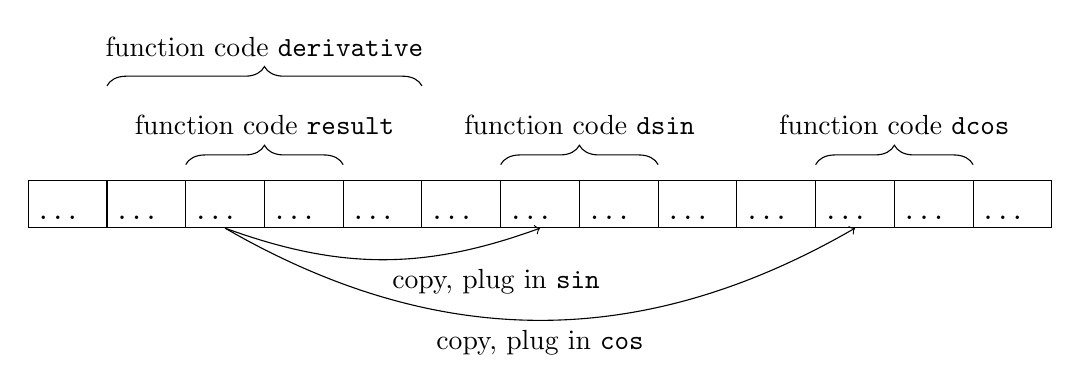
\begin{tikzpicture}
  [ 
    cell/.style={text width=8mm,
      text height=4mm, draw=black, inner sep=1mm},
    ld/.style={draw=blue,shorten >=2pt,->}
  ]
  \node  (a0) at ( 0,0) [cell] {\ttfamily ...};
  \node  (a1) at ( 1,0) [cell] {\ttfamily ...};
  \node  (a2) at ( 2,0) [cell] {\ttfamily ...};
  \node  (a3) at ( 3,0) [cell] {\ttfamily ...};
  \node  (a4) at ( 4,0) [cell] {\ttfamily ...};
  \node  (a5) at ( 5,0) [cell] {\ttfamily ...};
  \node  (a6) at ( 6,0) [cell] {\ttfamily ...};
  \node  (a7) at ( 7,0) [cell] {\ttfamily ...};
  \node  (a8) at ( 8,0) [cell] {\ttfamily ...};
  \node  (a9) at ( 9,0) [cell] {\ttfamily ...};
  \node (a10) at (10,0) [cell] {\ttfamily ...};
  \node (a11) at (11,0) [cell] {\ttfamily ...};
  \node (a12) at (12,0) [cell] {\ttfamily ...};
  
  \draw [decorate, decoration={brace,amplitude=7pt}, xshift=-0pt, yshift=0pt]
  		( 0.5, 1.5) -- ( 4.5, 1.5) node [midway, yshift=+0.5cm] 
		(braceFuncDerivative) {function code \texttt{derivative}};
	
  \draw [decorate, decoration={brace,amplitude=7pt}, xshift=-0pt, yshift=0pt]
  		( 1.5, 0.5) -- ( 3.5, 0.5) node [midway, yshift=+0.5cm] 
		(braceFuncResult) {function code \texttt{result}};
		
  \draw [decorate, decoration={brace,amplitude=7pt}, xshift=-0pt, yshift=0pt]
  		( 5.5, 0.5) -- ( 7.5, 0.5) node [midway, yshift=+0.5cm] 
		(braceFuncResult) {function code \texttt{dsin}};
		
  \draw [decorate, decoration={brace,amplitude=7pt}, xshift=-0pt, yshift=0pt]
  		( 9.5, 0.5) -- (11.5, 0.5) node [midway, yshift=+0.5cm] 
		(braceFuncResult) {function code \texttt{dcos}};
		
	\draw [->, bend right=20]
		(a2.south) to node 
		[below right=0] {copy, plug in \texttt{sin}} 
		(a6.south);
  
	\draw [->, bend right]
		(a2.south) to node 
		[below] {copy, plug in \texttt{cos}} 
		(a10.south);
\end{tikzpicture}
\end{center}
\end{tcolorbox}
%
\end{frame}

% =========================================================================== %

\begin{frame}[fragile]
%
\begin{columns}[T]
\column{.5\linewidth}
\begin{Large}
	{Lambdas}
\end{Large}
\vspace{6pt}
\begin{itemize}
\item Shorthand form for very simple functions
\item Often: \enquote{single-use functions}, parameters to other functions
\item Example: choose sorting criterion (see next slide)
\item Obey same rules as \enquote{normal} functions (scopes, treatment of mutable/immutables, optional/variadic/... arguments, ...)
\end{itemize}
%
\column{.5\linewidth}
\begin{codebox}[Syntax: Lambdas]
\begin{minted}[fontsize=\scriptsize]{python}
var = lambda args : expression(args)
\end{minted}
\end{codebox}
%
\begin{codebox}[Equivalent Code]
\begin{minted}[fontsize=\scriptsize]{python}
def var (args) :
    return expressio(args)
\end{minted}
\end{codebox}
%
\begin{codebox}[Syntax: Calling Lambdas]
\begin{minted}[fontsize=\scriptsize]{python}
result = var(args)
\end{minted}
\end{codebox}
\end{columns}
%
\end{frame}

% =========================================================================== %

\begin{frame}[fragile]
%
\begin{codebox}[Example: Sort Strings by Length]
\begin{minted}[fontsize=\scriptsize, linenos]{python}
stuffToSort = ["Vicki wollte ins Script",
               "epsilon", 
               "Darf Ich Das Behalten"
              ]

stuffToSort.sort(key = lambda element : len(element))

print(stuffToSort)
\end{minted}
\end{codebox}
%
\begin{cmdbox}[Output: Sort Strings by Length]
\begin{minted}[fontsize=\scriptsize]{text}
['epsilon', 'Darf Ich Das Behalten', 'Vicki wollte ins Script']
\end{minted}
\end{cmdbox}
%
\begin{hintbox}[Sorting criterion (\texttt{key})]
\texttt{key} is a lambda that computes a number (rank) from each element in the container. The elements in the container then are sorted according to this rank.
\end{hintbox}
%
\end{frame}

% =========================================================================== %

\begin{frame}{Recursion}
%
\begin{itemize}
\item Functions can call other functions and in particular, can call \emph{themselves}
\item Each call creates an \enquote{closed box}: To each call there is a proper set of variables
\item Useful for solving \emph{self-similar} problems
	\begin{itemize}
	\item Problem can be decomposed into sub-problems
	\item A sub-problem has the same form as the main problem, but:
	\item The amount of data to process is smaller, and:
	\item There is at least one trivial case, and:
	\item All sub-problems can be decomposed into a set of trivial problems
	\end{itemize}
\end{itemize}
%
\begin{hintbox}
To understand recursion, you first need to understand recursion.
\end{hintbox}
%
\end{frame}

% =========================================================================== %

\begin{frame}[fragile]{Example: Sum over Elements in a List}
%
Of course, we know that this problem can be easily solved with \inPy{total = sum(someList)}. Here, however, we want to illustrate the technique recursion. Hence, we'll follow this idea:

\vspace{-4pt}
\begin{tcolorbox}[title=Recursive Approach]
The sum over the elements in a list is equal to its first element plus the sum over the remaining elements.
\end{tcolorbox}
%
\begin{codebox}[Implementation: Recursive Array Sum]
\begin{minted}[fontsize=\scriptsize, linenos]{python}
def recSum (data) :
    if len(data) == 1 : return data[0]
    else              : return data[0] + recSum(data[1:])
    
print(recSum(list(range(4))))    # Ausgabe: 6 = 0 + 1 + 2 + 3
\end{minted}
\vspace{-4pt}
\end{codebox}
%
\end{frame}

% =========================================================================== %

\begin{frame}[fragile]
%
\begin{codebox}[Implementation: Recursive Array Sum]
\begin{minted}[fontsize=\scriptsize, linenos]{python}
def recSum (data) :
    if len(data) == 1 : return data[0]
    else              : return data[0] + recSum(data[1:])
    
print(recSum(list(range(4))))    # Ausgabe: 6 = 0 + 1 + 2 + 3
\end{minted}
\end{codebox}
%
\begin{codebox}[Call (line 5) sends to level 0, width=.7\linewidth, nobeforeafter, equal height group = B]
\scriptsize\inPy{data = [0, 1, 2, 3]}
	\begin{codebox}[Level 0 (line 3) sends to level 1]
	\scriptsize\inPy{data = [1, 2, 3]}
		\begin{codebox}[Level 1 (line 3) sends to level 2]
		\scriptsize\inPy{data = [2, 3]}		
		\end{codebox}
	\end{codebox}
\end{codebox}
%
\begin{hintbox}[Regard, width=.29\linewidth, nobeforeafter, equal height group = B]
Each level \enquote{lives} in its own scope! The symbol \texttt{data} refers to different locations in memory! All of them exist in parallel!
\end{hintbox}
%
\end{frame}

% =========================================================================== %\\

\begin{frame}[fragile]
%
	\begin{codebox}[Evaluation{,} level 0]
		\begin{codebox}[Evaluation{,} level 1]
			\begin{codebox}[Evaluation{,} level 2]
				\begin{codebox}[Evaluation{,} level 3]
				\scriptsize\inPy{return 3   # 0th element in [3]}
				\end{codebox}
				\scriptsize\inPy{return 2 + 3   # 0th element in [2, 3] plus result of recSum, level 3}
			\end{codebox}
			\scriptsize\inPy{return 1 + 5   # 0th element in [1, 2, 3] plus result of recSum, level 2}
		\end{codebox}
		\scriptsize\inPy{return 0 + 6   # 0th element in [0, 1, 2, 3] plus result of recSum, level 1}
	\end{codebox}
%
\end{frame}

% =========================================================================== %\\


\begin{frame}{Remarks}
%
\begin{itemize}
\item Maximum recursion depth (by default): 1000
\item A lot of overhead -- slow execution
\item But: \emph{some} problems can be solved extremely efficiently that way
	\begin{itemize}
	\item [\thus] \emph{Exercise}
	\item [\thus] Lecture \emph{Algorithmen und Datenstrukturen} (each summer term, Prof. Stefan Solbrig)
	\end{itemize}
\item Maths says: any recursive algorithm can be implemented \emph{iteratively}
\item Reality says: \emph{This is darn hard!}
\end{itemize}
%
\end{frame}
\end{document}

% MAREI!!
% whom do I give credit? Where?